%% Plantilla para el documento de investigación, este sera el archivo maestro
%% Por: Patricia Elizabeth Romero Rodríguez
%% Fecha inicio : 5 de marzo de 2014,

\documentclass[11pt]{report}
\usepackage[utf8]{inputenc}
\usepackage[spanish]{babel}
\inputencoding{utf8}
\usepackage{ragged2e}
\usepackage{graphicx}% Include figure files
\graphicspath{ {figures/} }
\usepackage{dcolumn}% Align table columns on decimal point
\usepackage{latexsym}
\usepackage{bm}% bold math
\usepackage{makeidx}
\usepackage{amsmath}
\usepackage{multirow, array} % para las tablas
\usepackage{float} % para usar [H], se tiene que instalar un componente adicional, (para que no cambie de lugar la figura)

\usepackage{pdflscape}   %tablas en forma o la tablahorizontal
\usepackage{amssymb}
\usepackage{listings} % para los listados de código fuente

\usepackage{anysize} % Permite emplear cualquier medida de márgenes.
\marginsize{3cm}{2cm}{2cm}{3cm}% Controla los márgenes {izquierda}{derecha}{arriba}{abajo}.

\parindent=1.5cm
\parskip=1em

\usepackage{longtable}

\def\contentsname{͍NDICE}
\def\listfigurename{͍NDICE DE FIGURAS}

\newtheorem{ejem}{Listado}
\newtheorem{teor}{Teorema}
\newtheorem{defi}{Definición}

\begin{document}

\justify
\pagenumbering{roman} \setcounter{page}{1}

%\include{dedicatoria}
%\include{agradecimientos}

%\include{resumen} % hacer la ficha resumen al final
\tableofcontents

\newpage
\listoffigures
%\newpage
\listoftables

\newpage
\pagenumbering{arabic} \setcounter{page}{1}

%\chapter{Introducción}
\noindent Para el desarrollo de software se debe considera aspectos que influyen en el precio que debe pagar el usuario final como ser: Costo de desarrollar el software, Costo de mantenimiento, Costo del entorno de ejecución,  Costo por agregar nuevas características, el número de usuarios a utilizar el software, y el modelo de distribución que define como es que el usuario final va adquirir el producto y las nuevas versiones. 

\section{Descripción del problema}
\noindent En el negocio de desarrollo de software de propósito general o comercial, los costos de desarrollo, mantenimiento, tener  entornos de ejecución (servidor) por el lado del cliente y la distribución del producto son determinantes para definir el precio que el usuario pagara por el producto.

\noindent A continuación se describe situaciones que afectan el incremento del precio del software:

\begin{itemize}
   	\item Instalación y actualización del software en diferentes lugares geográficos, lo cual hace que el proveedor tenga un soporte técnico para la puesta en ejecución y 	 las respectivas actualizaciones del software en los ambientes de ejecución de los clientes. Por otro lado los clientes que pueden ser empresas necesitan tener un departamento de Tecnología e Información que administre los ambientes de ejecución, agregando recursos de hardware a medida que pueda ir necesitando el software.
    \item Los clientes no siempre pueden llegar a tener la última actualización, algunos podrían estar trabajando con versiones anterior y esto hace que el proveedor tenga que dar soporte técnico a estas versiones.
    \item Agregar nuevas características al software también puede ser un factor determinante en cuanto al tiempo y costo que puede tomar.

\end{itemize}

\noindent Actualmente el desarrollo de software está siendo enfocado a ofrecer servicios en la nube (internet) donde usuarios potenciales puedan usar el software sin la necesidad de instalar en sus equipos. Esta manera de que el usuario final pueda acceder y utilizar el software, se lo denomina “Software como un servicio – Software as a Service (Saas)”, El cual es un modelo de distribución de software.

\section{Objetivos}
\noindent En este proyecto de grado, se pretende alcanzar los siguientes objetivos:

\subsection{Objetivo General}

\noindent Implementar un Software como un servicio, optimizando los recursos en el proceso de desarrollo del software. 


\subsection{Objetivos Específicos}

\noindent Para lograr el objetivo General, se pretende realizar los siguientes objetivos específicos:
\begin{itemize}
  \item Aplicar la metodología 12factor en las diferentes etapas de AUP, para el desarrollo de un Software como un Servicio – SaaS.
  \item Hacer uso de un servicio en la nube que proporcione  infraestructura en hardware y software para los entornos de ejecución. De tal forma que se puede aumentar o disminuir los recursos de acuerdo a la demanda (número de clientes que usan el software).
  \item Implementar un modelo que defina, la automatización de instalación de ambientes de desarrollo, construcción de ejecutable, verificación de los cambios nuevos en el código no afecte a funcionalidades ya definidas anteriormente, y la puesta en ejecución de la aplicación.
\end{itemize}

\section{Justificación}
\noindent En este proyecto de grado se pretende justificar en los siguientes ámbitos:
\begin{itemize}
  \item \textbf{Metodológico:} Se pretende plantear un modelo para optimizar el proceso de desarrollo hasta la puesta en ejecución de la aplicación. Considerando aspecto de: versionamiento de código, automatizar la preparación de entornos de desarrollo y ejecución e Integración continua.
  \item \textbf{Social}: Una guía para estudiantes o profesionales que se están introduciendo o se dedican al desarrollo de software. Como caso de estudio, se ha considerado realizar una aplicación web para la administración de pedidos en mototaxis que sera de mucha ayuda para las empresas dedicadas en éste rubro.
  \item \textbf{Tecnología}: Como plataforma principal se pretende usar Nodejs que define una arquitectura manejado por eventos – Event Driven lo cual permite crear aplicaciones escalables.
\end{itemize}

\section{Limites y Alcances}
\noindent En el proyecto de grado se pretende enfocar más al proceso de desarrollo del software y la puesta en ejecución. Para lo cual se define los siguientes límites y alcances:
\begin{itemize}
  \item No se realizara un estudio de costo. Se realizara un enfoque más a los factores que pueden afectar al costo de producto.
  \item Los factores que se consideraran son: desarrollo del software, distribución, ambientes de ejecución, y el mantenimiento.
  \item Para los ambientes de ejecución, se utilizara servicios en la nube como ser heroku o docker. De tal forma que no sea necesario instalar o preparar un servidor.
  \item En el caso de estudio. El software como un servicio será estándar para todas las empresas del mismo rubro. Lo que significa que no se podrá extender o agregar nuevos complementos para personalizar en las diferentes empresas.
\end{itemize}

\section{Diseño metodológico}
\noindent La metodología 12factor definida por [Adam Wiggins, 2012], está enfocada para el desarrollo de aplicaciones SaaS (Software as a Service). Esta metodología trata de que en el proceso de desarrollo del software se cumpla ciertos objetivos, los cuales son:

\begin{itemize}
  \item Tener una configuración automatizada para los entornos de desarrollo, puesta en ejecución de la aplicación.
  \item La aplicación debe ser portable entre los diferentes entornos de ejecución.
  \item Tener un conjunto de herramientas para la puesta en ejecución de la aplicación en plataformas en la nube.
  \item La aplicación debe ser escalable de tal forma que se realicen mínimos cambios de herramientas, arquitectura, o prácticas de desarrollo.
\end{itemize}

\noindent Para lograr los objetivos citados anteriormente, la metodología 12factor se enfoca en los siguientes puntos: 
\begin{itemize}
  \item Código base: Versionamiento de codigo en un repositorio central.
  \item Dependencias: Explícitamente declarar y aislar dependencias.
  \item Configuración: La informacion de conexion a base de datos, servicios externos, credenciales, configuracion de entornos de ejecucion. 
  \item Servicios externos que utiliza la aplicación: tener los servicios externos como recursos adjuntos que pueden ser cambiados en cualquier momento.
  \item Construcción, lanzamiento, y puesta en ejecución: Tener las etapas de construccion, lanzamiento y puesta en ejecucion independientemente. 
  \item Procesos: Poder ejecutar la aplicacion en un o mas procesos. 
  \item Enlazamiento a puerto: los servicios de la aplicacion deben estar expuesto atraves de un puerto.
  \item Concurrencia: Definir un modelo arquitectonico que soporte escalabilidad
  \item Minimizar el tiempo de inicio y apagado de la aplicacion: Despliegue rapido de codigo o cambios de configuracion y la puesta en ejecucion en los ambientes de produccion.
  \item Paridad entre los ambientes de desarrollo y producción: despliegue de cambios de un ambiente a otro sea rápido, al momento de trabajar en arreglar errores o problemas que se dieron en produccion.
  \item Registro de eventos. Logs: Nos permite tener un registro de lo sucedido cuando se presenta un problema de la aplicacion que esta disponible para los usuarios.
  \item Administración de procesos: para incrementar las instancias de la aplicacion dependiendo a la frecuencia de usuarios esten usando la aplicacion al mismo tiempo, Proceso de migracion de bases de datos, ejecucion de script para la validacion de cambios en el codigo fuente.
\end{itemize}

\noindent La metodología AUP se enfoca en el desarrollo de aplicaciones usando técnicas agiles como ser Desarrollo dirigido por pruebas,  Modelo Ágil, Gestión de Cambios Ágil.

\noindent La metodología AUP define las siguientes etapas:

\begin{itemize}
  \item \textit{Inicialización:} Identificación del alcance del proyecto, definir una potencial arquitectura.
  \item \textit{Elaboración:} Proveer una arquitectura más clara del software.
  \item \textit{Construcción:} Implementación del software basados en las características de prioridad alta para los inversionistas. 
  \item \textit{Transición:} La validación de software y la puesta en ejecución en los ambientes de producción.
\end{itemize}

\noindent Principios de la metodología AUP:
\begin{itemize}
  \item \textit{Modelo:} Comprensión de las reglas de negocio, plantear diseños de solución para los problemas de dominio.
  \item \textit{Implementación:} transformar los modelos, diseños en código y ejecutar un básico nivel de pruebas (pruebas de unidad).
  \item \textit{Pruebas:} Realización de evaluaciones para asegurar la calidad del producto.
  \item \textit{Puesta en ejecución:} desplegar el software en los ambientes de producción y que esté disponible para los usuarios finales.
  \item \textit{Administración de configuración:} Administración de los artefactos del proyecto y versiones.
  \item \textit{Administración del Proyecto:} manejo de riesgos, direccionamiento de personas.
  \item \textit{Entorno:} se enfoca en las necesidades del equipo de desarrollo, que se está siguiendo el proceso (estándares y guías), herramientas (hardware, software, etc.).
\end{itemize}

\begin{figure}[ht]
  \centering
  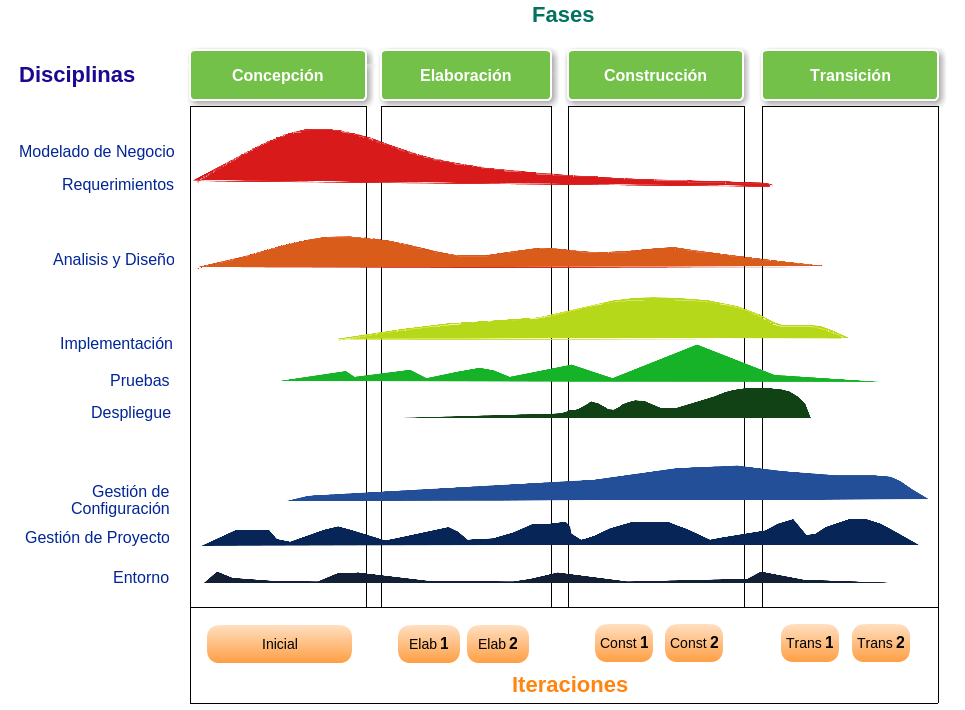
\includegraphics[width=15cm, height=9cm]{chapter1-aup-stages.png}
  \caption{Aplicación de las disciplinas en las fases del Proceso Unificado Agil AUP [Elaboracion propia ]}  
\end{figure}

\begin{figure}[ht]
  \centering
  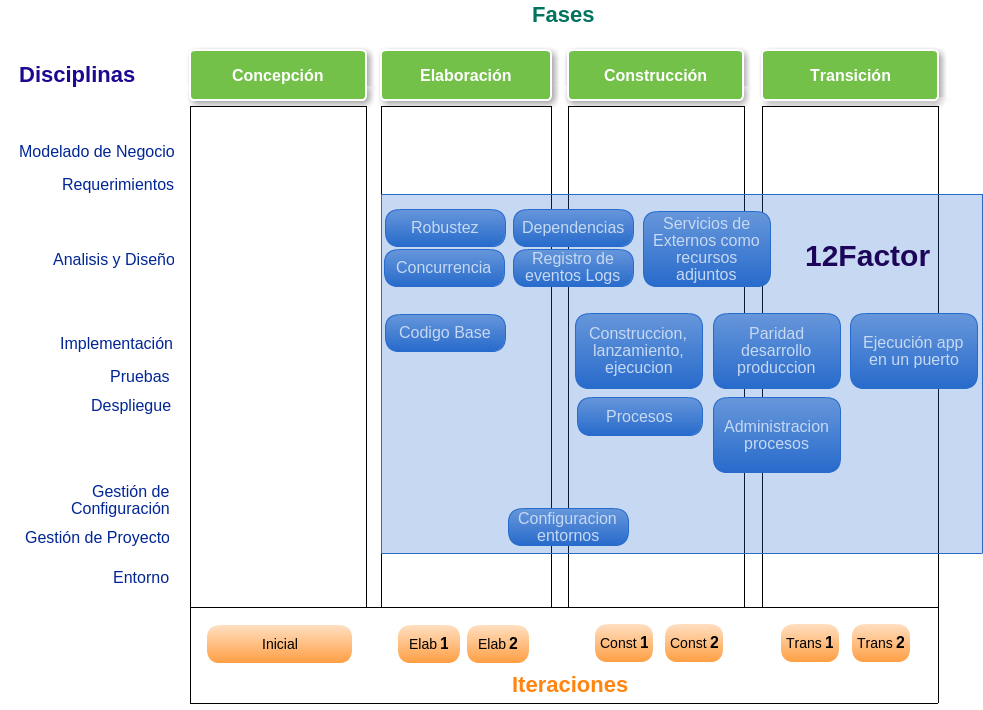
\includegraphics[width=15cm, height=9cm]{chapter1-model-12factor-aup.png}
  \caption{12factor introducida en las disciplinas de AUP en las diferentes fases (Elaboración propia)}  
\end{figure}

\begin{figure}[ht]
  \centering
  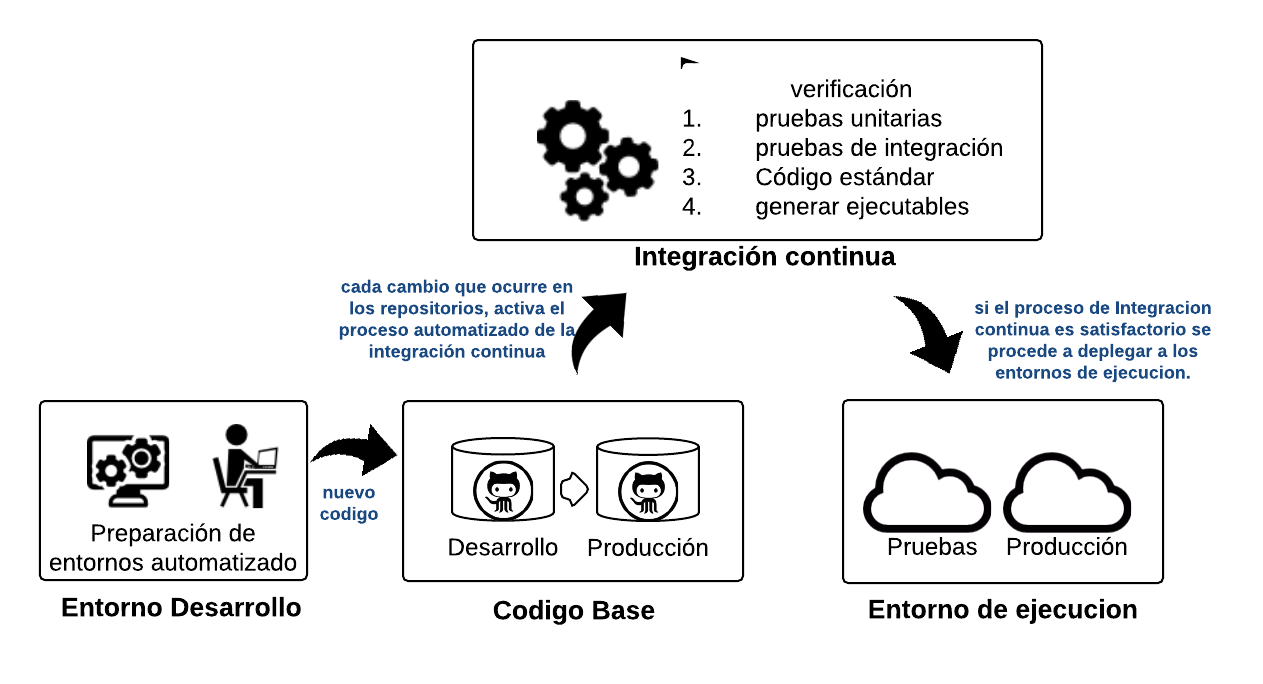
\includegraphics[width=12cm, height=6cm]{chapter1-model-process-development.png}
  \caption{Automatización de procesos, desde la preparación de ambientes de desarrollo, validacion de cambios en el codigo base y despliegue de los cambios en los ambientes de ejecucion (Elaboración propia)}  
\end{figure}
\noindent Tener tareas automatizadas en el proceso de desarrollo del software como ser: preparación de entornos de desarrollo para nuevos desarrolladores, validación de nuevas caracteristicas o arreglo de errores, introducida al codigo base. Verificando si se esta siguiendo el codigo estandard definida por el equipo de desarrollo, ejecución de test unitarios y de integracion, generacion de ejecutables y la puesta en ejecucion. Aceleran el proceso desarrollo del software y aseguran que los cambios introduciodos al codigo base, sean de incremento de tal forma que las nuevas caracteristicas no afecten a las anteriores.




 % este capítulo se hará en base al perfil,
\chapter{Factores a considerar en el desarrollo de software}
\noindent El desarrollo de software puede tener altos niveles de complejidad, mucho va ha depender del tipo de software que se quiere desarrollar, el modelo de negocio al cual está enfocado, la precisión en las funcionalidades del software, los tiempos de respuesta, la usabilidad para los usuarios finales.
\noindent La ingeniería de software está enfocado a desarrollo de software, por lo cual es necesario tomarlo en cuenta. Según [Roger S. Pressman, 2010] “La ingeniería de software abarca un proceso, una colección de métodos (práctica) y una gran variedad de herramientas que permiten a los profesionales construir software de alta calidad.”


\section{Proceso de desarrollo de Software}
\noindent El proceso de desarrollo define un marco de trabajo, donde se tiene como entrada las necesidades o requerimientos de los clientes y dentro del proceso se tiene un conjunto de actividades que nos permiten llegar a construir el producto.

\noindent Entre las principales actividades que se tiene en el proceso de desarrollo segun [Sommerville, 2005] son:
\begin{itemize}
  \item Especificación del Software: Donde los clientes y personas involucradas definen los requerimientos y sus restricciones del  Software.
  \item Desarrollo del Software: Donde el software se diseña y construye.
  \item Validación del Software: Donde se valida de que el software desarrollado cumple con las exigencias y expectativas del cliente.
  \item Evolución del Software: Donde el software tiene a cambiar y adaptarse a los nuevos requerimientos del cliente.
\end{itemize}

\begin{figure}[ht]
  \centering
  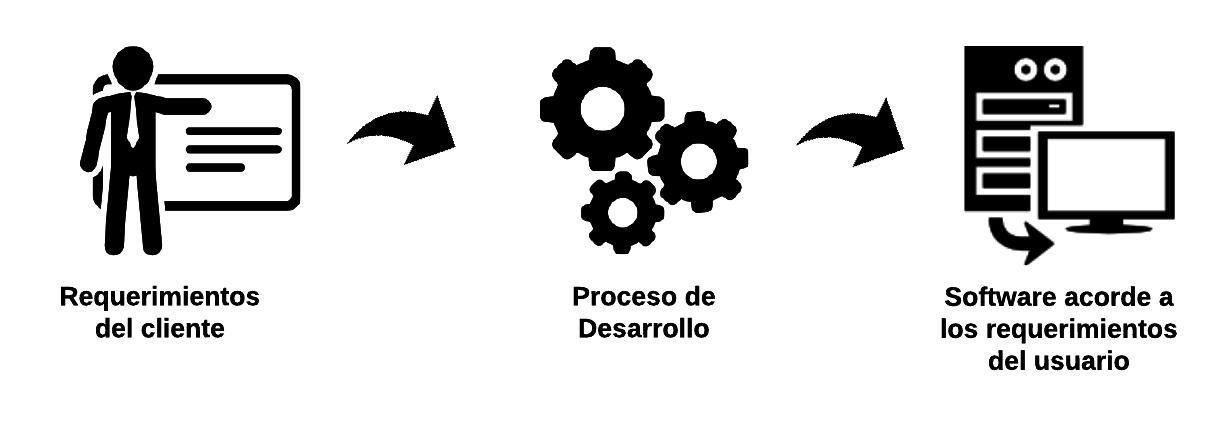
\includegraphics[width=12cm, height=4cm]{chapter2-process-software-development.png}
  \caption{Descripcion grafica del proceso de desarrollo [Elaboración propia]}  
\end{figure}

\noindent El proceso de desarrollo del software tiene que ir mejorando en conjunto al desarrollo del producto, tiene que ir solucionando las debilidades o necesidades que se pueden tener a medida que se va desarrollando el producto.
 
\section{Modelo del Proceso de Desarrollo de software}
\noindent El Modelo del proceso de desarrollo de software es una representación del proceso que se quiere aplicar para el desarrollo del software. En el modelo se define y se puede ver claramente el flujo de trabajo e interacción de las personas involucradas en cada actividad o etapa dentro del desarrollo de software.
\noindent Los Modelos pueden incluir actividades que son parte de los procesos y productos de software y el papel de las personas involucradas en la ingeniería del software. Algunos de los modelos que se pueden tener segun [Sommerville, 2005] son:
\begin{itemize}
\item Un modelo del flujo de trabajo: En este modelo se tiene el flujo de actividades humanas en el proceso junto a sus entradas, salidas y dependencias.
\item Un modelo del flujo de datos o actividades: En este modelo se tiene el conjunto de actividades y el tratamiento de datos que realiza cada actividad.
\item Un modelo de roles:En este modelo se tiene el conjunto de roles y responsabilidades de las personas involucradas en el proceso de desarrollo.
\end{itemize}

\noindent Los modelos de proceso de desarrollo pueden variar de acuerdo a los siguientes factores:
\begin{itemize}
\item Enfoque de desarrollo: Modelo en cascada, espiral, iterativo e incremental.
El tipo de software que se quiere desarrollar: aplicación de escritorio, plugin, aplicación web de propósito general.
\item mantenimiento de versiones: Si el software en desarrollo va a tener versiones o solo sera una unica version al mismo tiempo.
\item manifiesto de paradigmas de programación: Se puede tener modelos que estén reforzados con manifiesto o metodologías para el desarrollo del software.
\end{itemize}
\noindent Se debe tener mucho cuidado en adaptar un modelo, no se puede forzar el uso del modelo dentro el desarrollo del software.   

\section{Confiabilidad, Escalabilidad y Mantenimiento}
\noindent Los productos de software segun [Martin Kleppmann, 2014] tienen un cierto número de atributos asociados que reflejan la calidad de ese software. Estos atributos no están directamente asociados con lo que el software hace, Más bien, reflejan su comportamiento durante la ejecución, la estructura y organización del código fuente y la documentación asociada.

\subsection{Confiabilidad}
\noindent La confiabilidad se da en las interacciones que realiza el usuario final en la aplicación y que la aplicación pueda responder a las expectativas del usuario. La aplicación tiene que ser tolerante a fallos o a posibles errores que pueda cometer el usuario, debe poder responder de forma adecuada a situaciones inesperadas. El tiempo de respuesta debe ser lo más razonablemente posible. La seguridad en el acceso a información de los usuarios debe ser controlada, de tal forma que el usuario sepa que su información está segura y que las personas autorizadas puedan entrar.


\subsection{Escalabilidad}
\noindent La escalabilidad es la habilidad del software desarrollado, de poder adaptarse a incrementos de carga. Para decir que un software es escalable, se debe analizar su comportamiento con cierto número de usuarios que utilizan el software de forma simultánea e ir incrementando el número de usuarios para conocer la variación que se da en cuanto a los tiempos de respuesta y como se comporta el software en las diferentes situaciones.
\noindent Para poder tener una aplicación escalable, se debe definir el patrón de arquitectura a utilizar. La interacción de las capas definidas en el software, deben ser lo más vertical posible. Se debe tener un balance de carga que optimiza el uso de recursos de hardware. 

\subsection{Mantenimiento}
\noindent El costo del software no se refleja al inicio de desarrollo del software, sino en la etapa de mantenimiento, arreglando errores, manteniendo el software en operación, investigando fallas, adaptando el software a nuevas plataformas tecnológicas, pagando deudas técnicas y agregando nuevas características.
Para reducir el costo y la dificultad de mantenimiento de un software, se debe tomar particular atención a tres principios de diseño para un software.
\begin{itemize}
\item Operabilidad: la puesta en ejecución, monitorio, manejo de logs deben de lo más fácil posible para la administración operativa del equipo.
\item Simplicidad: Los nuevos desarrolladores deberían de poder integrarse al proyecto y comprenderlo sin complicaciones.
\item Plasticidad:Los ingenieros en el futuro puedan hacer cambios en el software, de tal forma que solo se modifique la parte que se quiere (cambiar de tecnología o módulo).
\end{itemize}

\section{Integración Continua}
\noindent Una definicion de Integracion Continua por [Martin Fowler, 2006] \"Integración Continua es una buena práctica en el desarrollo de software, donde los miembros del equipo integran su trabajo con frecuencia, lo cual conduce a múltiples integraciones por dia\". Cada integración se verifica por una construcción automatizada que valida los cambios realizados a través de criterios de validación como ser:
- Ejecución de pruebas automatizados
- Código estándar
- porcentaje de Cobertura de las pruebas unitarias en el código fuente.

\section{Distribución del software}
\noindent in progress

\section{Software como un Servicio}
\noindent in progress

\section{Ambientes de ejecución}
\noindent in progress
 % lo que se llama el marco teórico, es un sistema de conceptos
%\chapter{Concepción}
\noindent En este capítulo se pretende describir el caso de estudio, los requerimientos funcionales, requerimientos técnicos, criterios de aceptación del entregable de esta iteración y la aplicación de la metodología 12 factor en las diferentes fases de Proceso Unificado Ágil-AUP.

\section{Concepción}
\noindent El objetivo de esta fase es obtener una máxima compresión cliente - equipo de desarrollo. Los requerimientos funcionales, el alcance del software a desarrollar (criterios de aceptación) y la definición de la arquitectura de la aplicación.

\subsection {Modelado de Negocio}
\noindent Las empresas que ofrecen servicio de pedidos a domicilio a través de motorizados (mototaxis) en su mayor parte administran su negocio por medio de archivos Excel por lo cual tienen muchas limitaciones.
Entre las actividades administrativas que se realizan en este tipo de empresa es la siguiente:
\begin {itemize}
\item Registro de pedidos que se realizan a diario.
\item Registro y cobro de multas de inasistencia a los 	motorizados.
\item Registro y cobro por frecuenta a los motorizados.
\item La asignación de pedidos a los respectivos 	motorizados.
\end{itemize}
\section{Elaboración}
\section{Construcción}
\section{Transición}
%
\chapter{Elaboración}
\noindent En el presente capítulo se reforzará y se analizará la solución que se planteó en el capítulo anterior teniendo como resultado los siguientes elementos:

\begin{itemize}
\item Diseño de requerimientos
\item Diseño de la base de datos
\item Especificación Plan de pruebas
\item Entorno de Desarrollo
\item Proceso de Integración Continua
\item Plan de Iteraciones 
\end{itemize}

\noindent El objetivo de la fase de \textbf{Elaboración} en AUP - Proceso Unificado Ágil, es que el equipo de desarrollo profundice en la comprensión de los requisito del sistema y en validar la arquitectura propuesta en la fase de \textbf{Iniciación}.

\noindent Adicionalmente en este capítulo se ha considerado los siguientes elementos de la metodología 12 factor:
\begin{itemize}
\item Minimizar tiempo de encendido y apagado aplicación
\item Concurrencia
\item Código Base
\item Dependencias
\item Configuraciones
\end{itemize}

\section{Diseño de requerimientos}
\noindent A continuación de definen los diseños por cada módulo definido en la arquitectura presentada en el capítulo anterior. Para una mejor compresión se define por cada módulo: los diagramas de secuencia, diagramas de clases, diseño de interfaz gráfica y especificación de criterios de aceptación para las pruebas.

\subsection{Módulo de Pedidos}
\noindent El módulo de pedidos tiene como objetivo resolver los siguientes requerimientos:
\begin{itemize}
\item Registro de los pedidos realizados por los clientes (Req. \#1).
\item Asignación de pedidos a los motorizados de la empresa (Req. \#2).
\item Listar los pedidos realizados en el dia (Req \#3).
\end{itemize}

\begin{figure}[H]
  \centering
  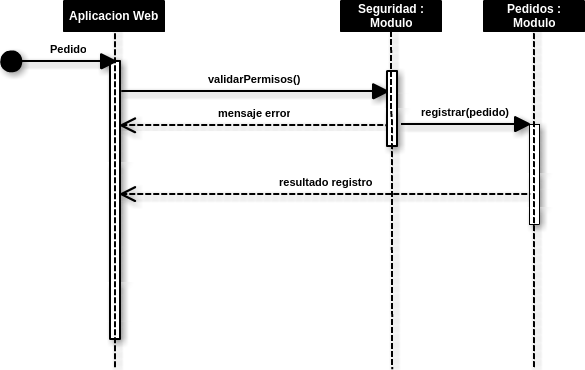
\includegraphics[width=11cm, height=8cm]{chapter4-register-customer-request-sequence-diagram.png}
  \caption{Registro de pedidos [Elaboración propia]}  
\end{figure}

\begin{figure}[H]
  \centering
  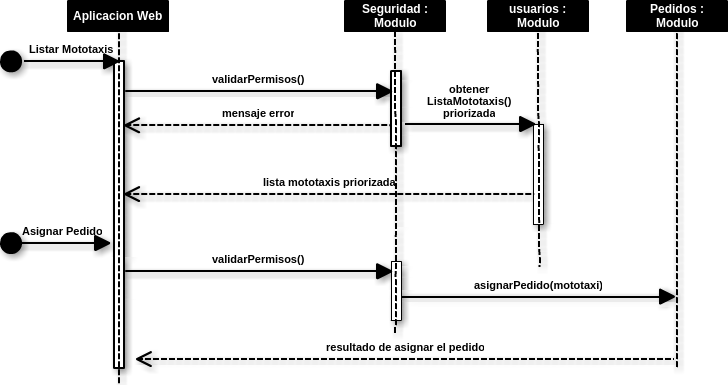
\includegraphics[width=12cm, height=8cm]{chapter4-assign-customer-request-sequence-diagram.png}
  \caption{Asignación de pedidos [Elaboración propia]}  
\end{figure}

\begin{figure}[H]
  \centering
  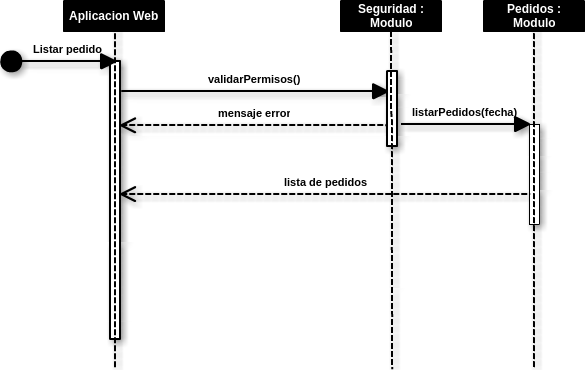
\includegraphics[width=11cm, height=8cm]{chapter4-get-list-customer-request-sequence-diagram.png}
  \caption{Obtener lista de pedidos [Elaboración propia]}  
\end{figure}


\begin{figure}[H]
  \centering
  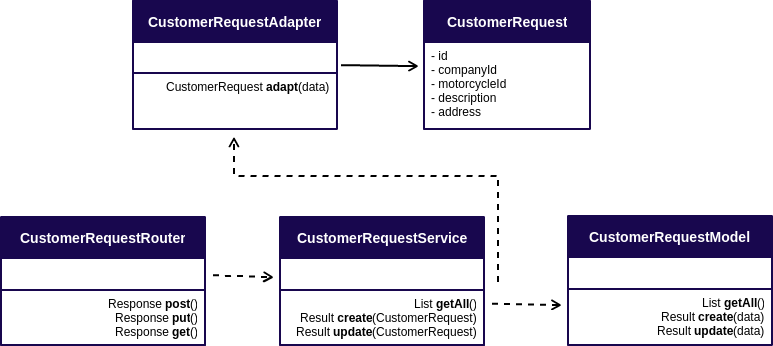
\includegraphics[width=14cm, height=7cm]{chapter4-customer-request-module-class-diagram.png}
  \caption{Diagrama de clases módulo de pedidos [Elaboración propia]}  
\end{figure}

\begin{figure}[H]
  \centering
  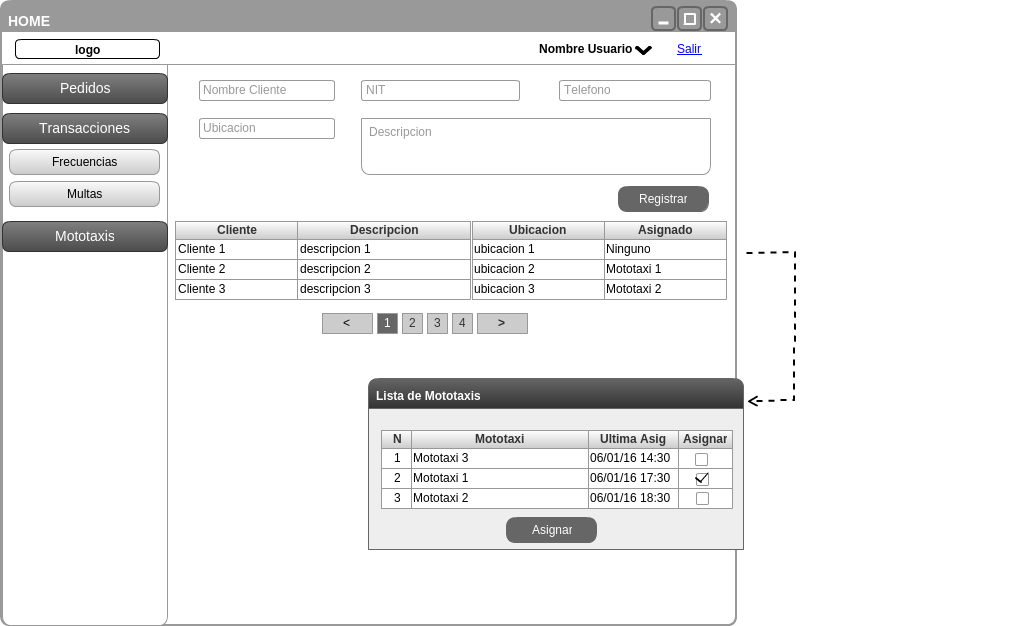
\includegraphics[width=22cm, height=15cm]{chapter4-customer-request-module-view-design.png}
  \caption{Diseño de la vista módulo de pedidos [Elaboración propia]}  
\end{figure}

\subsection{Módulo de Transacciones}
El módulo de transacciones tiene como objetivo resolver los siguientes requerimientos:
\begin{itemize}
\item Registrar el cobro por frecuencia diaria a los respectivos motorizados de la empresa (Req. \#5).
\item Registrar el cobro por multa de inasistencia de los respectivos motorizados de la empresa (Req. \#6).
\end{itemize}
\subsection{Módulo de Usuarios}
El módulo de Usuarios tiene como objetivo resolver los siguientes requerimientos:
\begin{itemize}
\item Registro de motorizados de la respectiva empresa (Req. \#4).
\item Listar los motorizados de la respectiva empresa (Req. \#7).
\item Registro de cuentas de operadores de la respectiva empresa (Req. \#8).
\item Ver ingresos diarios y mensuales de los ingresos por cobro de frecuencia y multas (Req. \#9).
\item Actualizar datos de usuarios (Req. \#10).
\end{itemize}
\subsection{Módulo de Seguridad}
\noindent El módulo de Seguridad tiene como objetivo resolver los siguientes requerimientos:
\begin{itemize}
\item Autenticación de usuarios y mostrar la información de acuerdo al perfil usuario (Req. \#11).
\item Control permisos de accesos a los recursos de información de acuerdo al perfil de usuario (Req. \#12).
\item Control de acceso a los usuarios que solo puedan acceder a la información de la empresa a la cual pertenecen (Req. \#13).
\item Permitir crear solo una cuenta administrador por empresa (Req. \#14).
\item Permitir cambiar contraseña (Req. \#15).
\end{itemize}

\section{Diseño de la base de datos}
\noindent Para el diseño de la base de datos se ha considerado las sugerencias descritas en [mongoDB data model design, 2014] para la elaboración de un modelo de datos en mongodb donde se puede tener modelos de datos embebidos y/o modelo de datos normalizados.

\noindent La estructura de una base de datos en mongodb está compuesta por las colecciones (tablas sql). En una colecciones se almacenan los documentos (filas sql), los documentos son objetos en formato json que almacenan la información en clave-valor.

\begin{figure}[H]
  \centering
  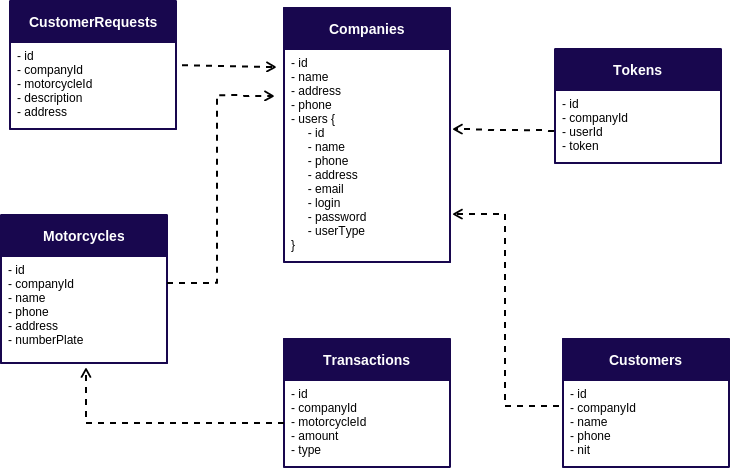
\includegraphics[width=14cm, height=8cm]{chapter4-database-design.png}
  \caption{Colecciones de la base de datos [Elaboración propia]}  
\end{figure}

\section{Entorno de Desarrollo}

\section{Proceso de Integración Continua}



 

%\include{cap5}
%\include{Pruebas y/o experimentación}
%\include{Conclusiones}

% En formato APA 
\chapter*{Referencias Bibliográficas\markboth{Referencias Bibliográficas}{Referencias Bibliográficas}}

\begin{itemize}
	\item \textbf{Adam Wiggins} (2013). \textit{La metodologia \textit{\textbf{twelve factor app}} esta enfocada a la construccion de Software como un servicio.} Disponible en \small{http://12factor.net/}. Fecha de consulta: 29 de noviembre 2015.
	\item \textbf{Ian Sommerville} (2005). \textit{Ingenieria de Software (S\'{e}ptima edici\'{o}n)}. Pearson Addison Wesley.  
    \item \textbf{Martin Kleppmann} (2014). \textit{Designing Data-Intensive Applications}. O'REILLY
    \item \textbf{Martin Fowler} (2006). \textit{Continuos Integration} Disponible en \small{http://www.martinfowler.com/}. Fecha de consulta: 06 de diciembre 2015.
    \item \textbf{Roger S. Pressman} (2010). \textit{Software Engineering \textit{\textbf{A Practiticioner's Approach}}}. McGraw-Hill Disponible en \small{http://www.webcourses.ir/dl/Software-Engineering.pdf}. Fecha de consulta: 06 de diciembre 2015.
    \item \textbf{Saas manifiesto} (2010). \textit{The Real SaaS Manifest\'{o}} how it can benefit your business. Workday Inc. Disponible en \small{http://www.cio.co.uk/cmsdata/whitepapers/3437477/workday-the-real-saas-manifesto-whitepaper-uk.pdf}. Fecha de consulta: 09 de diciembre 2015.
    \item \textbf{SWEBOK} (2014). \textit{Guide to the Software Engineering Body of Knowledge}. IEEE Computer Society.
	\item \textbf{Leonard Richardson \& San Ruby} (2007). \textit{RESTful Web Services.} O’REILLY. Disponible en \small{http://restfulwebapis.org/restful\_web\_services.pdf}. Fecha de consulta: 27 de diciembre 2015.
\end{itemize}




% Aquí empiezan los anexos
%\appendix
%\include{AnexoA} % manual de usuario
%\include{AnexoB} % minigosario de términos
%\include{evidencias}

\end{document}
